\documentclass[a4paper,man,natbib, floatsintext]{apa7}

\usepackage[english]{babel}
\usepackage[utf8x]{inputenc}
\usepackage{amsmath}
\usepackage{graphicx}
\usepackage[colorinlistoftodos, textsize=scriptsize]{todonotes}

% Added by us
\usepackage{caption}
\usepackage{lipsum}
\usepackage{float}
\usepackage{tikz}
\usepackage{tikz-qtree}
\usepackage{lscape}
\usepackage{multicol}
\usepackage{makecell}
\usepackage{array}
\usepackage{color, colortbl}
\usepackage{xr}
\externaldocument[sm-]{SM}
\newcolumntype{P}[1]{>{\centering\arraybackslash}m{#1}}
\newcommand{\YL}[1]{\textcolor{blue}{YL: #1}}
\newcommand{\YLDEL}[1]{\sout{\textcolor{black}{YL: #1}}}
\newcommand{\dieuwke}[1]{\textcolor{green!60!black}{DH: #1}}
\newcommand{\dnote}[1]{\todo[color=green!40, inline]{DH: #1}}
%
\renewrobustcmd{\bfseries}{\fontseries{b}\selectfont}
\renewrobustcmd{\boldmath}{}
\newrobustcmd{\B}{\bfseries}

\title{Mechanisms for handling nested agreement dependencies in neural language models and humans}

\shorttitle{Nested dependencies in NLMs and humans}
\author{-}
\affiliation{-}


\abstract{Recursive processing in sentence comprehension is considered a hallmark of human linguistic abilities. However, its underlying neural mechanism in the human brain remains largely unknown. Neural Language Models (NLMs) have recently shown remarkable success on various linguistic tasks. As currenlty the only non-human computational system capable of accomplishing such tasks, NLMs suggest new opportunities to study neural mechanisms underlying natural language processing, which might give insights about similar processes in humans. We use subject-verb number agreement as an index of syntactic processing in NLMs and investigate the neural mechanisms underlying processing of nested agreements --- a prototypical case of recursive structures. We found that a neural agreement mechanism in the model can successfully handle outermost agreements of nested constructions, however, albeit shorter, the model makes more errors on embedded dependencies, and dramatically fails when the embedded dependency is long-range. We derive predictions about human performance based on these error patterns in NLMs and on properties of its agreement mechanism and test them in a behavioral experiment. Results show that unlike NLMs, humans do not exhibit a dramatic failure on long-range embedded dependencies. However, overall, error patterns of humans and NLMs are remarkably similar, suggesting NLMs as compelling models for sentence processing that can account for various effects in human data. To test whether the main discrepancy is quantitative (e.g., dependent on the number of nesting) or qualitative (e.g., due to recursive processing unique to humans), we conclude by listing testable predictions for future experiments.}
\keywords{Grammatical agreement, Neural Language Models, Long-Range Dependencies, Recursion, Syntactic processing, Recurrent Neural Networks, Relative Clauses.}

\begin{document}
\maketitle
\section{Introduction}

% \input{figures/fig_design.tex}

\begin{itemize}
\item Neural language models (NLMs) are wonderful blah blah blah, revived interest in
  looking at them as computational models of language processing
\item Current research in the area focuses on understanding the behaviour of NLMs wrt
  various grammatical phenomena; some work showing correlations
  between internal states and said phenomena
\item Number agreement is an area where some steps have been taken
  towards mechanistic understanding:
  \begin{itemize}
  \item sparse feature-propagation mechanism controlled by distributed
    grammar network
  \end{itemize}
\item Our goal here is two-fold:
  \begin{itemize}
  \item First, we replicate our earlier results on the emergence of
    this mechanism in a different language, as well as extending them to a different
    agreement phenomenon (\textbf{do we?}) confirming it is no fluke
  \item Second, we use our understanding of of how agreement is
    performed by NLMs to make a new prediction about a difficulty in agreement
    processing in humans (analogy to DiCarlo's work in vision?)
  \end{itemize}
\item Main result: the predicted pattern is confirmed; however, in other ways,
  human and NLM patterns differ, confirming that studying NLMs is
  productive, but the right perspective is not to treat them as
  full-fledged cognitive models, but rather as powerful computational
  systems that, when faced with challenges similar to those
  encountered by humans, might adopt partially analogous solutions
\end{itemize}

\section{Processing of a Single Subject-Verb Dependency in NLMs}
In the classic number agreement task (NA-task), subjects are presented with the beginning of a sentence (aka, `preamble') that contains a long-range subject-verb relation, such as: ``The keys to the cabinet\ldots'', and are asked to predict the verb to follow (e.g., ``are''). Human subjects make more agreement errors (e.g., continuing the preamble  above with ``is'' instead of ``are'') when the intervening noun (aka, `attractor') has a different grammatical number than the main subject (as in the preamble above, with plural subject ``keys'' and singular attractor ``cabinet'') . Behavioral measures collected during agreement tasks, such as error-rates, vary as a function of the syntactic environment of the long-range dependency. This has provided rich data to test hypotheses regarding online syntactic processing in humans \citep[e.g., ][]{franck2002subject, franck2006agreement, franck2007syntactic}.

Starting with the influential work of \citet{Linzen:etal:2016}, a growing
literature \citep[e.g.,][]{Gulordava:etal:2018, Bernardy:Lappin:2017,
  Giulianelli:etal:2018, Kuncoro:etal:2018a,Linzen:Leonard:2018,jumelet2019analysing} has
tested NLMs on the NA-task at the behavioural level, showing that these models have performance
and error patterns partially resembling those of humans.
More recently, we investigated the underlying neural mechanism of an
English NLM during the processing of a long-range dependency
\citep{lakretz2019emergence}. We identified a neural circuit in the
network that encodes and carries grammatical number across long-range
dependencies, showing also that processing in NLMs is sensitive to the
structure of the subject-verb dependency. In the next section we
describe the main findings of our previous study, followed by a replication of them in a NLM trained on Italian. 

\YL{Add something of the sort - readers that are familiar with previous findings can also safely continue to the next section.}


\subsection{Agreement in the English NLM}

\subsubsection{The Noun-PP Number-Agreement Task}
The main NA-task used by \citet{lakretz2019emergence} contained sentences with a subject-verb dependency separated by a prepositional phrase (e.g., ``The \textbf{boy} near the car \textbf{smiles}''), referred to as the `Noun-PP' task. This task comprises four conditions, which correspond to the four possible assignments of grammatical number to the main subject and attractor (SS, SP, PS and PP; S-singular, P-plural). The NLM was presented with preambles of sentences from this task, and predictions of the model of the next word were then extracted, from which error-rates were computed (Methods). 

\subsubsection{Long-Range Number Units}
Having verified that the network could predict the correct number with high accuracy, \citet{lakretz2019emergence} tested whether there were units in the network that were crucial to carry grammatical number across long-range dependencies.  To identify such units, \citet{lakretz2019emergence} conducted an ablation study, by removing a unit of the NLM at a time, and re-evaluating its performance on the Noun-PP NA-task. The ablation revealed that two (out of 1300) units in the network each caused a reduction in agreement performance towards chance level when ablated. One of these units only affected performance when the main subject of the sentence was singular, and was therefore called the `singular unit'. The other unit had an effect with plural subjects only, hence, the `plural unit'. 
No other unit had a comparable effect on network performance when ablated. A visualization of state dynamics of the singular and plural units confirmed their role in encoding and carrying through grammatical number across long-range dependency, robustly also in the presence of an attractor \citep[figure 1 in][]{lakretz2019emergence}.

\subsubsection{Syntax Units}
Since the activity of the long-range number units follow the structure of the syntactic long-range dependency, \citet{lakretz2019emergence} tested whether other units in the network encode syntactic information and inform the long-range number units about when to store and release number information in their encoding. Several units were found to have activity that is predictive about transient syntactic properties of the sentence. In particular, the activity of one of these `syntax' units followed the structure of the main subject-verb dependency, consistently across various sentence constructions \citep[figure 3 in][]{lakretz2019emergence}. 

\subsubsection{Short-Range Number Units}
\citet{lakretz2019emergence} further found that grammatical number information was also encoded
by other units in the network. Number information can still be
decoded from network activity even when the long-range number units
are removed. However, number information encoded in these other units is short-lived. Whenever new grammatical number information is
introduced (e.g., upon encountering a noun or a verb), activity in
these units abruptly switches to represent this last encountered
number. These `Short-Range Number Units' can therefore only support number-agreement dependencies that do not
enfold attractors (e.g., "The \textbf{boy} gracefully
\textbf{smiles}"). The presence of short-range number units explain why ablating the long-range circuit only affects agreement in long-distance dependencies.


\subsection{Agreement in the Italian NLM}
The choice to focus on Italian instead of English is based on two main reasons reasons. First, we found that the Italian NLM made available by \citet{Gulordava:etal:2018} achieves better performance than the English NLM on nested construction, which are computationally more demanding compared to sentences in the Noun-PP NA-task explored in \citet{lakretz2019emergence}. This might be explained by that Italian is morpho-syntactically richer than English. Second, in English, the plural is identical to the unmarked form of the verb, which can occur as infinitive, in first and second person, and often as a noun. This makes the occurrence statistics unbalanced, in favor of plural. \footnote{\citet{Gulordava:etal:2018} made available models in English, Italian, Hebrew and Russian, which were optimized by conducting a grid search, and became since a subject of research in several subsequent studies \citep{Giulianelli:etal:2018, jumelet2019analysing, wilcox2018rnn, futrell2019neural}. We therefore did not consider repeating the optimization process in these or other languages and used the same set of hypterparameters reported by this study when training additional NLMs (methods). Given the above considerations, Hebrew and Italian might have been also good alternative for the purpose of this study. \YL{not sure if all this is really needed}.}

To test whether the Italian NLM has developed an agreement mechanism similar to the model trained on English, we followed the same steps described in the previous section - an ablation study, visualization of unit dynamics and a connectivity analysis.

\subsubsection{Ablation Results Reveal a Long-Range Number Unit} To identify unit(s) that encode grammatical number for long-range dependencies, we conducted an ablation study on the Italian model made available by \citet{Gulordava:etal:2018}, following the steps described above, using an Italian noun-PP NA-task (Methods). We found that the ablation of one unit from the second layer of the network, unit 815, led to a significant reduction in performance in both incongruent conditions (figure S1).\footnote{We repeated the ablation experiment also with another 19 NLMs that we trained on the same corpus and found that most models showed a significant reduction in performance after unit ablation, for only a few units, with some models showing a significant effect on the SP or PS condition only, and others on both (figure S2).}

\subsubsection{Dynamics of the Number Unit Show Robustness to Attractors} 
To confirm that unit 815 is a long-range number unit, we visualized the dynamics of the unit during the processing of the long-range dependency, by extracting its activations during the processing of all sentences in the noun-PP NA-task. Figure \ref{fig:nounpp}A describes the resulting average cell-state activations. It shows that number information is robustly encoded throughout the subject-verb dependency, also in the presence of an attractor (dashed lines). Furthermore, the dynamics of unit 815 show that it encodes both singular and plural number, using negative and positive cell activations, respectively.

\subsubsection{Efferent Weights of the Number Unit are Clustered with Respect to Number}
Finally, we extracted the efferent weights of unit 815, which project onto the output layer. Figure S2A shows that unit 815 deferentially affects unit activations in the output layer, depending on whether they represent singular or plural forms of the verb. This is consistent with its role as a number unit. In what follows, we refer to unit 815 as the long-range `Number Unit'.

\subsubsection{Long-Range Gender Units are Also Found in the Network }
Agreement in Italian can also occur with respect to gender, for instance, in sentences containing predicative adjectives: ``\textbf{Il bambino} accanto al madre \`{e} \textbf{bello}'' (``The boy near the mother is pretty''), in which the subject and adjective agree with respect to both number and gender. We therefore hypothesized that there should also exist long-range `gender' units in the network, with dynamics that are robust to possible attractors (e.g., to "madre" above, which is feminine). Using an NA-task with adjective phrases and repeating the ablation study (Methods), we found that one unit dramatically reduced the performance of the NLM when ablated, and its inner-state dynamics showed robust encoding across the subject-adjective dependency (Figure \ref{fig:nounpp}A), also in the presence of attractors (dashed lines). Connectivity analysis further confirmed that the efferent weights of the long-range `gender' unit were clustered with respect to whether they project to masculine or feminine adjective words in the output layer (figure S2B).

\vspace{10pt}
In sum, these results extend previous findings to another language and another grammatical feature. Similarly to English, only a few long-range number units emerged in the Italian NLMs during training, in the majority of the cases. The NLM has developed a similar encoding scheme for both grammatical number and gender, independently. Taken together, this shows that sparse long-range feature units consistently emerge in NLMs.

\YL{(we may need to specify that our lexicon included only biological gender, or repeat the experiments with also inanimates.)}. 

\begin{figure}
    \centering
    \includegraphics[width=\textwidth]{figures/model_activations_nounpp.png}
    \caption{\textbf{Cell activity of the number unit (panel A) and gender unit (panel B) during the processing of a single long-range dependency across a prepositional phrase:} four conditions are presented, corresponding to whether the main subject of the sentence is singular (red curves) or plural (blue), and to whether the main subject (`bambino') and the intervening noun (`contadino') have the same (congruent) or opposite number (incongruent)}
    \label{fig:nounpp}
\end{figure} 

\section{Processing of Two Subject-Verb Dependencies in NLMs and Humans}
The core mechanism to carry agreement information across long-range dependencies in NLMs involves a very small number of units--one (Italian) or two (English). This mechanism was shown to robustly process sentences having a single long-range dependency. We next ask: given that the long-range agreement mechanism is sparse, and can thus only encode a single number feature at a time, how will the NLM process \emph{two} long-range dependencies that are active at once?

Two simultaneously active long-range dependencies occur in various constructions, such as center-embedded nested dependencies, a prototypical example of recursion. In nested dependencies, once the long-range agreement mechanism is engaged in tracking the main dependency, there may be no more suitable units available to process the \textit{embedded} agreement. For example, in the sentence ``The \textbf{boy} that the \textit{farmer} near the \underline{fathers} \textit{watches} \textbf{knows} the daughters'', there are two grammatical numbers that need to be carried across a long-range dependency: (1) that of the main subject `boy', and (2) that of the embedded subject `farmer'. Once the NLM  encounters the main subject, its grammatical number can be stored through the long-range agreement mechanism up to the main verb `knows'. However, during this period, since the mechanism is already taken up, once the embedded subject `farmer' is presented to the network, there is no robust way to encode and carry its number up to the embedded verb `watches'. The NLM is thus predicted to fail to process the embedded dependency in nested structures.

We emphasize two conditions for this predicted failure:
\begin{itemize}
	\item The two dependencies are \textit{simultaneously} active at some point: if this is not the case, i.e., the dependencies are successive (e.g., ``The \textbf{boy} near the \underline{cars} \textbf{says} that the \textit{farmer} near the \underline{fathers} \textit{watches} the daughters''), the long-range mechanism can first complete processing the first dependency, and then reset before encoding the next one. 

        \item Both dependencies are \textit{long-range}: in the case
          of a short-range dependency nested within a long-range one
          (e.g., ``The \textbf{boy} that the \textit{farmer}
          \textit{watches} \textbf{knows} the daughters''), the
          embedded short-range dependency can still be processed by
          the short-range units we described above, although possibly
          in a less robust way.
\end{itemize}


\subsection{Experimental Design}
To test the hypothesis that the sparsity of the long-range mechanism can lead to a significant processing difficulty at the embedded dependency, we created a two-by-two design that manipulates the above two conditions: (1) whether the two dependencies are \textit{successive} or \textit{nested}, and (2) whether the embedded dependency is \textit{short} or \textit{long} range. Figure \ref{fig:design} describes the resulting four NA-tasks: Short-Successive, Long-Successive, Short-Nested and Long-Nested ('Short' and 'Long' therefore refer to the length of the embedded dependency only). 

The successive tasks serve as control. They minimally differ from the nested ones up to the embedded verb, by only a single word (`dice' (`says') in figure \ref{fig:design}). Note also that tasks that have a long embedded dependency have a third noun, which functions as a possible attractor, inside the embedded dependency. We will refer to this most-deeply embedded noun as the attractor, although technically the subjects of the main and nested clauses can also act as attractors on each others' verbs.

For each NA-task, we generated various \textit{conditions} by varying the number of the main and embedded subject noun, and that of the attractor. Short-Successive and Short-Nested have each four conditions corresponding to the possible assignments of number to the main and embedded subjects - SS, SP, PS and PP. Similarly, Long-Successive and Long-Nested have eight conditions, based on the possible numbers of the main, embedded subject and attractor - SSS, SSP, SPS, etc. In what follows, by \textit{congruent subjects} we refer to conditions in which the main and embedded subjects share grammatical number (SS, PP, SSS, SSP, PPS and PPP), and by \textit{incongruent subjects} to the rest (SP, PS, SPS, etc.). By \textit{congruent attractor}, we refer to conditions in which the embedded subject and the third noun share grammatical number (SSS, SPP, PSS and PPP), and by \textit{incongruent attractor} to conditions in which they differ (SSP, SPS, PSP, PPS) (Methods).

Several studies reported markedness effects in agreement, whereby humans make more errors when the grammatical number of the attractor is plural. This effect was reported in several languages and in both comprehension and production (English: \citet{Bock:Miller:1991, eberhard1997marked, wagers2009agreement, lago2015agreement}; Italian: \citet{vigliocco1995constructing}). \textbf{(Didn't Lago et al also report the effect in Spanish? Or did they just limit themselves to the plural-attractor case based on their English results? Also, aren't there studies on French showing the effect? Perhaps the Vigliocco paper?} Since we use error rates as an index of processing difficulties across various conditions, we strove to increase their overall signal. Therefore, we conducted all analyses on contrasts with a plural attractor. Results for the full set of conditions, with both singular and plural attractors, are reported in the SM.

Table \ref{tbl:predictions} summarizes our predictions for each task and structure, while ignoring for now, for ease of presentation, differences among specific conditions. For Short- and Long-Successive, no significant processing difficulties are predicted, since the long-range mechanism can encode the main and nested grammatical numbers sequentially. For Short- and Long-Nested, the long-range mechanism is predicted to successfully process the main dependency and therefore no significant difficulties are predicted on the main verb (beyond the relative difficulty to process center-embeddings reported for both humans \citep{traxler2002processing} and NLMs \citep{marvin2018targeted}). In contrast, the embedded dependency in Short-Nested cannot rely on the long-range agreement mechanism, as it is recruited by the main dependency. Consequently, the processing of the embedded dependency can only rely on short-range mechanisms, which might not be as robust as the long-range ones. We are thus agnostic about success in this case. Finally, in Long-Nested, the performance on the embedded verb is predicted to be significantly low, given that the long-range mechanism can process only a single agreement, as described above. \YL{After re-reading this paragraph, we could also consider omitting it. Marco: I think it's useful, I just shortened it.}


\begin{center}
\begin{table}
\centering
\begin{tabular}{|P{3.5cm}||P{3.5cm}|P{3.5cm}|}
    \hline
    \B Sentence Type & \B Main Verb & \B Embedded Verb \\
    \hline
    Successive-Short & Good  & Good \\
    \hline
    Successive-Long & Good & Good \\
    \hline
    Nested-Short & Good & - \\
    \hline
    Nested-Long & Good & Poor \\
    \hline
\end{tabular}
\caption{A summary of the predictions of model performance on successive and nested dependencies based on the sparsity of the long-range mechanism. Cell values represent the degree of predicted performance on the agreement task. Due to possible compensation mechanisms carried by the short-range number units, we make no precise predictions regarding performance on the embedded verb of Nested-Short.}
\label{tbl:predictions}
\end{table}
\end{center}

\begin{figure*}
    \centering
    \includegraphics[width=\textwidth]{figures/design.png}
    \caption{\textbf{A full-factorial design for two subject-verb dependencies}. Human subjects and Neural Language Models (NLMs) were presented with sentences from four different syntactic structures, which all have two subject-verb dependencies: a main dependency (continuous lines) and an embedded dependency (dashed). The first factor of the design determines whether the two dependencies are \textit{successive} (top structures) or \textit{nested} (bottom), depending on whether the structure has a sentential complement or an object-extracted relative clause, respectively. The second factor determines whether the embedded dependency is \textit{short} (left side) or \textit{long} (right). We refer to the four resulting structures as: Short-Successive, Long-Successive, Short-Nested, Short-Long.}
    \label{fig:design}
\end{figure*}

\subsection{Results for the Italian NLM}
\subsubsection{The Number Unit Shows Sequential Processing of Two Successive Dependencies and Robust Encoding of the Main Dependency in Nested Constructions}
We first simulate NLM dynamics for all NA-tasks and conditions, by presenting all sentences from each condition to the NLM (methods \ref{}). Figure \ref{fig:2by2_dynamics} presents hidden-state dynamics of the long-range number unit during the processing of all conditions from the four NA-tasks. We note that, consistent with results on a single dependency, the grammatical number of the main subject is encoded with the same polarity as found in the Noun-PP task - positive for plural (blue) and negative for singular (red). Second, in successive NA-tasks, the activation of the number unit returns to baseline after encountering the main verb ('dice'), and then rises back once the main subject is encountered. This shows that the number unit can sequentially encode two grammatical numbers in two successive dependencies, also when the two numbers are opposite. In particular, note that in Long-Successive, the grammatical number of the embedded subject is robustly carried across the attractor ('fratello') in the incongruent conditions (dashed lines). Finally, in both Short- and Long-Nested, the grammatical number of the main subject is robustly carried across the main dependency up to the main verb ('evita') \YL{fix xticklabels}, and in particular, across the embedded subject and verb that carry an opposite number in some conditions (dashed lines).

\begin{figure*}
    \centering
    \includegraphics[width=\textwidth]{figures/model_activations.png}
    \caption{\textbf{Dynamics of the hidden activation of the number unit during the processing of two subject-verb dependencies.} Number-unit activity is presented for the four structures in the design: Short-Successive (panel A), Long-Successive (B), Short-Nested (C) and Long-Nested (D). For each structure, results are presented for the four conditions, corresponding to whether the main subject of the sentence is singular (red curves) or plural (blue), and to whether the main and embedded subjects have the same grammatical number (congruent; continuous lines) or not (incongruent; dashed lines).}
    \label{fig:2by2_dynamics}
\end{figure*}


\subsubsection{NLM Performance on Successive Dependencies}
Since no significant processing difficulty is predicted in the successive tasks, we conduct the experiments on the embedded agreement only, which is expected to be the more difficult one. This allowed us to reduce experimental duration in the parallel study with human participants. Also, to facilitate the interpretation of the results, we group conditions by whether the main and embedded subjects are congruent or not.

Figure \ref{fig:SC_results}A presents the resulting NLM error rates (figure S2 further provides the full error-rate distribution across all conditions). Several effects are observed in the results: 

\begin{itemize}
    \item \textbf{Near to perfect performance on all conditions}: Overall, for both Short- and Long-Successive, the performance of the NLM was found to be almost error free (\YL{add stats}), with slightly more errors in the Long-Successive case (\YL{add stats}). 
    \item \textbf{Subject-congruence effect}: We next tested for a \textit{subject-congruence effect}, i.e., whether incongruent-subject elicited more errors compared to congruent ones. We found significant subject-congruence effect in both Short- and Long-Successive (Short-Nested: $z-value=5.4, p-value<0.001$; Long-Nested: $z-value=6.4, p-value<0.001$). \textbf{Maybe emphasize that there is an effect, but it's based on comparing very high accuracies?}
\end{itemize}
 
\subsubsection{NLM Performance on Nested Dependencies}
Figure \ref{fig:objRC_results}A presents the corresponding error-rates in the case of nested dependencies (figure S3 shows the full error-rate distribution across all conditions). Several effects are observed in the results:

\begin{itemize}
    \item \textbf{Incongruent conditions elicit more errors}: a significant subject-congruence effect was found on both the embedded and main verbs, in both Short- and Long-Nested (Short-Nested main: $z-value=93.1, p-value<0.001$; Short-Nested embedded: $z-value=50.9, p-value<0.001$; Long-Nested main $z-value=67.0, p-value<0.001$; Long-Nested embedded: $z-value=120.5, p-value<0.001$). In all cases, incongruent subjects elicited more errors compared to congruent subjects.
    \item \textbf{Processing of embedded verbs is more error-prone}: for both Short- and Long-Nested, a significant interaction was found between subject-congruence and verb-position (embedded/main), with a larger increase of error rate due to incongruent subjects on the embedded compared to the main verb (Short-Nested: $z-value=32.3, p-value<0.001$; Long-Nested: $z-value=84.2, p-value<0.001$).
    \item \textbf{A longer embedded dependency is more error prone}: for errors made on the embedded verb, we found a significant interaction between subject-congruence and the length of the embedded dependency (Short/Long-Nested), with a larger increase of error-rate due to incongruent subjects in Long-Nested ($z-value=7.4, p-value<0.001$).
\end{itemize}
 
\vspace{10pt}

\subsubsection{Discussion of NLM results}
Focusing on cases with incongruent subjects, the error patterns of the NLM are overall consistent with the predictions summarized in table \ref{tbl:predictions}. First, successive dependencies are relatively easy for the model, and can be processed sequentially. This is consistent with the sequential encoding observed in the dynamics of the number unit (figure \ref{fig:2by2_dynamics}), which shows a robust encoding of grammatical number of embedded subjects, also in the presence of an attractor. Second, the main dependency in both Short- and Long-Nested was successfully processed (i.e., significantly better than chance level), although with more overall errors compared to successive dependencies. Third, the NLM made an exceptionally large number of errors on the embedded verb in Long-Nested, as predicted by the sparsity of the long-range mechanism. This is prominent in the case of incongruent-subject, since only then the grammatical number of the main subject encoded in the long-range mechanism can interfere. Finally, the NLM made a relatively large number of errors on the embedded verb in Short-Nested but was significantly better than chance level ($error-rate = 0.5$; \YL{stats}). The reduced number of errors in Short- compared to Long-Nested is consistent with the findings about a short-range mechanism that can process the embedded dependency, compensating for the momentary recruitment of the long-range mechanism for the main one. 

\YL{refer to the effect of the attractor in SM}.

\subsection{Results for Humans}
The previous section has shown that the NLM cannot robustly encode two long-range dependencies that are active at once. The NLM was found to: (1) make an increased error rate on the embedded verb in both Short- and Long-Nested, and (2) to make an exceptionally high error-rate in the latter case, when the embedded dependency was long-range.

Suppose that a similarly sparse mechanism is also used by humans to carry number features through long-distance agreement structures. We derive the following predictions:

\begin{itemize}
    \item \textbf{Prediction 1}: humans will make more agreement errors on the embedded compared to the main dependency in the incongruent conditions of Long-Nested. 
    \item \textbf{Prediction 2}: humans will make more errors on the incongruent conditions of the embedded verb when the embedded dependency is long- compared to short-range.
\end{itemize}

Prediction 1 derives from the robustness of the agreement mechanism in processing the main but not the embedded dependency, as was observed in the NLM performance. Note that we we don't make precise predictions regarding Short-Nested, due to possible short-range compensation mechanisms in humans. Prediction 2 derives from the sparsity of the agreement mechanism and the dramatic failure of the model to process the embedded dependency in Long- but not Short-Nested. 

We tested these predictions by presenting Italian speakers with sentences from the same four NA-tasks in the design (figure \ref{fig:design}; Methods). In what follows, we describe the resulting agreement-error patterns in humans and then compare them to those of the NLM.

\subsubsection{Human Performance on Successive Dependencies}
Figure \ref{fig:SC_results}B presents the resulting error-rates for Short- and Long-Successive. 
\begin{itemize}
    \item \textbf{Relatively low error-rate}: humans made relatively few errors on successive constructions, although significantly above zero (\YL{stats}). Note that, in comparison to the Italian NLM, humans have a higher error baseline, to which unrelated factors that are specific to humans may contribute, such as occasional lapses of attention.
    \item \textbf{No subject-congruence effect}: we found no significant subject-congruence effect in Short-Successive, and a marginally significant subject-congruence effect in Long-Successive ($z-value=1.834, p-value=0.06$).
\end{itemize}
\YL{compare also to performance on noun-PP}.

\subsubsection{Human Performance on Nested Dependencies}
Figure \ref{fig:objRC_results}B presents errors-rate for Short- and Long-Nested. Several effects are observed in the results: 
\begin{itemize}
    \item \textbf{Subject-congruence effect on embedded and main verbs}: for both main and embedded verbs in both Short- and Long-Nested, incongurent subjects elicited more errors--a significant subject-congruence effect was found in all cases (Short-Nested main: $z-value=2.970, p-value=0.003$; Short-Nested embedded: $z-value=6.411, p-value<0.001$; Long-Nested main $z-value=3.630, p-value<0.001$; Long-Nested embedded: $z-value=7.274, p-value<0.001$).
    \item \textbf{Processing of embedded verbs is more error-prone}: for both Short- and Long-Nested, the increase in error rate due to incongruent subjects was larger for embedded compared to main verbs. A significant interaction was found between subject congruence and verb position in both cases (Short-Nested: $z-value=2.277, p-value = 0.02$, Long-Nested: $z-value=2.634, p-value = 0.008$).
    \item \textbf{A longer embedded dependency is more error prone}: for embedded verbs, the increase in error-rate due to incongruent subjects was comparable when the embedded long-range dependency was compared to the short one. No significant interaction was found between subject-congruence and length of the embedded dependency (Short- vs. Long-Nested).
\end{itemize}

    \subsubsection{Discussion of human results}
Overall, successive dependencies were, as expected, relatively easy for humans compared to nested ones. Subject-congruence effect was not found, or was marginally significant, which is consistent with sequential processing of grammatical number in NLMs. The results confirm \textit{Prediction 1}--the main dependency in both Short- and Long-Nested was less error prone than the embedded one, as was confirmed by a significant interaction between subject-congruence and verb position. However, although humans made more errors on the embedded dependency when it was long range, we did not find a significant interaction between subject-congruence and the length of the embedded dependency. Prediction 2 was therefore not confirmed by the results.

\vspace{10pt}
\YL{Add discussion. Decide whether to keep or remove the comparison table. Marco: I'm OK with removing the table. Also, I would leave a short discussion here, and defer a more extended discussion of similarities and differences to the conclusion.}
% Taken together, the results from the experiments show that there are key points of similarities between the agreement-error patterns produced by humans and NLMs. \ref{tbl:comparison} summarizes and compares these effects. As can be seen in the table, most of the key effects were found in both humans and NLMs. The main point of discrepancy regards subject-congruence effect on the main verb in nested constructions, which was found only for RNNs. We return to this point in the General Discussion, when we discuss interference dynamics in the model.

\begin{table}[h]
\tiny
\centering
\parbox{.4\linewidth}{
\centering
    \begin{tabular}{ |P{3cm}|P{1.3cm}|P{1.3cm}|  }
    \hline
    \rowcolor{cyan}
    \multicolumn{3}{|c|}{\textbf{Short-Successive}} \\
    \hline
    \rowcolor{cyan}
    \textbf{Effect} & \textbf{Humans} & \textbf{RNNs} \\
    \Xhline{3\arrayrulewidth}
    \rowcolor{green}
    \textbf{Subject Congruence (Embedded verb)} & X & X \\
    \hline
    
    \end{tabular}
}
\hfill
\parbox{.4\linewidth}{
\centering
    \begin{tabular}{ |P{3cm}|P{1.3cm}|P{1.3cm}|  }
    \hline
    \rowcolor{cyan}
    \multicolumn{3}{|c|}{\textbf{Long-Successive}} \\
    \hline
    \rowcolor{cyan}
    \textbf{Effect} & \textbf{Humans} & \textbf{RNNs} \\
    \Xhline{3\arrayrulewidth}
    \rowcolor{green}
    \textbf{Subject Congruence (Embedded verb)} & X & X \\
    \hline
    
    \end{tabular}
}

\vspace{25pt}

\parbox{.4\linewidth}{
\centering
    \begin{tabular}{ |P{3cm}|P{1.3cm}|P{1.3cm}|  }
    \hline
    \rowcolor{cyan}
    \multicolumn{3}{|c|}{\textbf{Short-Nested}} \\
    \hline
    \rowcolor{cyan}
    \textbf{Effect} & \textbf{Humans} & \textbf{RNNs} \\
    \Xhline{3\arrayrulewidth}
    \rowcolor{magenta}
    \textbf{Subject Congruence (Main verb)} & X &  V\\
    \Xhline{3\arrayrulewidth}
    \rowcolor{green}
    \textbf{Subject Congruence (Embedded verb)} & V &  V\\
    \hline
    \rowcolor{green}
    \textbf{Interaction: Subject-Congruence Verb-Position} & V &  V\\
    \hline
    
    \end{tabular}
}
\hfill
\parbox{.4\linewidth}{
\centering
    \begin{tabular}{ |P{3cm}|P{1.3cm}|P{1.3cm}|  }
    \hline
    \rowcolor{cyan}
    \multicolumn{3}{|c|}{\textbf{Long-Nested}} \\
    \hline
    \rowcolor{cyan}
    \textbf{Effect} & \textbf{Humans} & \textbf{RNNs} \\
    \Xhline{3\arrayrulewidth}
    \rowcolor{magenta}
    \textbf{Subject Congruence (Main verb)} & X &  V\\
    \Xhline{3\arrayrulewidth}
    \rowcolor{green}
    \textbf{Subject Congruence (Embedded verb)} & V &  V\\
    \hline
    \rowcolor{green}
    \textbf{Interaction: Subject-Congruence Verb-Position} & V &  V\\
    \hline
    
    \end{tabular}
}
\caption{A summary of all effects  humans and RNNs.}
\label{tbl:comparison}
\end{table}



\begin{figure*}[h]
    \centering
    \includegraphics[width=10cm]{figures/error_rates_successive.png}
    \caption{\textbf{Error rates on the Short- and Long-Successive:} collected from NLMs (panel A) and human subjects (B). Blue and red correspond to whether the main and embedded subjects agree on number (congruent subjects) or not (incongruent), respectively. Error bars represent standard error of the mean across all trials. ns - non significant. \textbf{Are these percentage values? Please specify.}}
    \label{fig:SC_results}
\end{figure*}


\begin{figure*}[h]
    \centering
    \includegraphics[width=10cm]{figures/error_rates_nested.png}
    \caption{\textbf{Error rates on the Short- and Long-Nested:} collected from NLMs (panel A) and humans subjects (panel B). Blue and red correspond to whether the main and embedded subjects agree in number (congruent subjects) or not (incongruent), respectively. Error bars represent standard error of the mean across all trials. ns - non significant.}
    \label{fig:objRC_results}
\end{figure*}


\section{Materials and Methods}

\subsection{NA-tasks}

\begin{table}
    \setlength\tabcolsep{2mm}
\small
\centering
\begin{tabular}{lll}
\multicolumn{3}{c}{\centering \textit{Finding number/gender units}}\\
\hline
\hline
\emph{Nounpp} & \texttt{\textbf{NP$_1$} prep NP$_2$ \emph{V}} & \specialcell{Il \textbf{ragazzo} accanto alla donna \emph{conosce}\vspace{-3mm}\\({\scriptsize The \textbf{boy} next to the woman \emph{knows}})} \\
   \emph{Nounpp-gender} & \texttt{det1 \textbf{N1} prep det2 N2 V \emph{ADJ}} & \specialcell{Il \textbf{ragazzo} accanto alla donna \'{e} \emph{basso}\vspace{-3mm}\\({\scriptsize \textbf{boy} next to the woman is \emph{short}})}\\
~\\
\multicolumn{3}{c}{\centering \textit{Nestedness experiments}}\\
\hline
\hline
\emph{Short-Successive} & \texttt{NP$_a$ V$_a$ che NP$_b$ V$_b$} & \specialcell{Il figlio dice che il \textbf{ragazzo} \emph{ama}\vspace{-3mm}\\{\scriptsize The son says that the \textbf{boy} \emph{loves}}} \\
\emph{Long-Successive} & \texttt{NP$_a$ V$_a$ che NP$_b$ P NP$_c$ V$_b$} & \specialcell{Il figlio dice che l'\textbf{amico} accanto al ragazzo \emph{conosce}\vspace{-3mm}\\{\scriptsize The son says that the \textbf{friend} next to the boy \emph{knows}}} \\
\emph{Short-nested} & \texttt{NP$_a$ che NP$_b$ V$_b$ V$_a$ } & \specialcell{Il \textbf{figlio} che il ragazzo osserva \emph{evita}\vspace{-3mm}\\{\scriptsize The \textbf{son} that the boy observes \emph{avoids}}} \\
\emph{Long-nested} & \texttt{NP$_a$ che NP$_b$ P NP$_c$ V$_b$ V$_a$} & \specialcell{Il \textbf{figlio} che la ragazza accanto ai padri ama \emph{evita}\vspace{-3mm}\\{\scriptsize The \textbf{son} that the girl next to the fathers loves \emph{avoids}}} \\
\end{tabular}
\caption{NA-tasks, \dieuwke{Add explanation. To save space, I used \texttt{NP} as an abbreviation for \texttt{Det N}. While this is of course an NP, it is also ab it confusing.}}
\end{table}

\subsection{Behavioral Experiment}
\subsubsection{Participants}
61 psychology students from the University of Milano-Bicocca (males = XX; Age = XX ± XX; Education = XX ± XX) took part in the experiment in exchange of course credits. Participants were Italian native speakers and were naive with respect to the experiment purpose. The study was approved by the ethical committee of the Department of Psychology, and ethical treatment was in accordance with the principles stated in the Declaration of Helsinki.

\subsubsection{Stimuli}
Stimuli comprised i) acceptable sentences; ii) violation trials, containing a number violation on the verb of one of the subject-verb agreements; iii) filler sentences, comprising several syntactic and semantic violations. 

Acceptable sentences were created using a pool of 10 nouns, 19 verbs, 4 prepositions (see table S1).
Starting from this pool of sentences, number-violation and filler trials were created by replacing either the main or embedded verb by the opposite form of the verb with respect to number. For example, ``il fratello che lo studente *accolgono ama i contadini'' (``the brother that the student *welcome loves the farmers'').

Filler trials contained either semantic violation or a syntactic violation that is not with respect for number. Syntactic violations were generated by either i) replacing to a verb in a wrong person, for example, ``il fratello che lo studente *accolgo ama i contadini''; ii) replacing a verb with a noun, for example, ``il fratello che lo studente *amica ama i contadini'' (the brother that the student *friend loves the farmers); iii) replacing a verb with its infinitive form, for example, ``il fratello che lo studente *accogliere ama i contadini'' (``the brother that the student *to welcome loves the farmers''). Semantic violations were generated by either replacing one of the noun with i) an inappropriate abstract one, for example, ``la *filosofia dice che la figlia ama la madre'' (the ``*philosophy says that the daughter loves the mother''); ii) inanimate noun, for example, ``la *matita dice che la figlia ama la madre'' (``the *pencil says that the daughter loves the mother''). To avoid correlation between abstract or inanimiate nouns and semantic violation, half of these filler trials were felicitous, for example, ``il padre dice che la figlia ama la *filosofia'' (``the father says that the daughter loves the *philosophy'', or ``il padre dice che la *matita appartiene alla figlia'' (``the father says that the *pencil belongs to the daughter''). See Supplementary Materials for more details.

In total, 540 sentences were presented to each participant, which were randomly sampled from a larger pool of sentences. From these, 180 sentences were acceptable, 180 with number violation, and 180 fillers. 

\subsubsection{Paradigm}
The experiment was conducted in two sessions (270 trials in each), which were performed by participants in different days. Each session lasted around 45 minutes. The two sessions took place at the same time of the day at a maximum temporal distance of two weeks. After receiving information about the experimental procedure, participants were asked to sign a written informed consent. 

Stimuli were presented on a 17” computer screen in a light-grey, 30-point Courier New font on a dark background. Sentences were presented using a Rapid Serial Visual Presentation (RSVP). Each trial started with a fixation cross appearing at the center of the screen for 600 ms, then single words were presented with SOA=500 ms, 250 ms presentation followed by 250 ms of black screen. At the end of each sentence, a blank screen was presented for 1500 ms, then a response panel appeared, with two labels “correct” and “incorrect”, on two sides of the screen (in random order each time) for a maximal duration of 1500 ms. A final screen, showing accuracy feedback was presented for 500 ms.

Participants were informed that they would be presented with a list of sentences which could be acceptable or containing a syntactic or semantic violation. They were instructed to press the “M” key of the Italian keyboard as fast as possible once they detected a violation. Sentences were presented up to their end even when participants pressed the button earlier. Then, in the response panel, participants were asked to press the “X” key if the sentence was correct, or “M” whether the sentence was not correct. During the entire session, participants were asked to keep their left index over “X” and their right index over “M” keys. After each trial participants received a feedback concerning their response: ``Bravo!'' (i.e. ``Good!'') in the case that sentence was correct, ``Peccato..'' (i.e. ``too bad...'') when it was incorrect. At the beginning of each session, participants performed a training block comprising XX items. The training section included all types of stimuli.

\subsubsection{Data and Statistical Analyses}
In ungrammatical trials, a violation could occur on either the main or embedded verb. Errors therefore correspond to trials in which a violation was missed. Since in ungrammatical trials a violation occurred on only one of the two verbs, the error can be associated with either the main or embedded dependency. In grammatical trials, errors correspond to trials in which participants reported a violation despite its absence. In contrast to ungrammatical trials, in which the violation marks the dependency, in grammatical trials it is not possible to associate an error with one of the two dependencies. Moreover, due to the presence of filler trials, the false detection of a violation could be unrelated to grammatical agreement (for example, a false detection of a semantic violation). Agreement errors were therefore estimated from ungrammatical trials only.

Statistical analyses were carried out using R, an open-source programming language \citep{R}. For each hypothesis testing, we fitted a mixed-effects logistic regression model \citep{Jaeger2008}, with participant and item as random factors, using the lme4 package for linear mixed effects models \citep{Bates}. Following \citet{Baayen:etal:2008}, we report the results from the model with the maximal random effects structure that converged for all experiments. 
%Data from participants with accuracy below 0.8 on the filler items were excluded from analyses.

\subsection{Language Model}
\subsubsection{Model Description}
The model architecture we use is identical to the architecture presented by \citet{Gulordava:etal:2018}. 
It consists of two layers with 650 Long-Short Term Memory (LSTM) units \citep{Hochreiter:Schmidhuber:1997}, input and output embedding layers of 650 units and input and output layers of size 50000 (the size of the vocabulary). The weights of the input and output embedding layers are not shared.
The last layer of the model is a softmax layer, whose activations sum up to 1 and as such corresponds to a probability distribution over all words in the NLM's vocabulary.

\subsubsection{Model Training} 
In addition to the NLM made available by \citet{Gulordava:etal:2018}, we train an additional 19 models using the same procedure and corpus (drawn from Wikipedia), giving 20 models in total. 
The models differ in the order in which those sentences are presented as well as the initialisation of their weights.
For all runs, we use a learning rate of 20, a batch size of 64 and a dropout rate of 0.2, the hyperparameters that \citet{Gulordava:etal:2018} reported to work best for this particular corpus and setup.
Following Gulordava et. al, but contrary to common practice in language modelling, we train the models on separate sentences, rather than longer pieces of discourse.
As common practice for training language models, we do not use an optimiser, but instead use a \emph{plateau-based} learning scheme, in which we half the learning rate whenever the validation perplexity of the model reaches a plateau.

\subsubsection{Model Evaluation} After training, we evaluate the resulting 20 models by considering their perplexity on a shared test set\footnote{\url{https://dl.fbaipublicfiles.com/colorless-green-rnns/training-data/Italian/test.txt}}. For the NA-tasks, following \citet{Linzen:etal:2016}, we compute accuracy by presenting the preamble of each sentence to the NLM and then compare the output probabilities assigned to the plural and singular forms of the verb. On each sentence, the model is scored 1 if the probability of the correct verb is higher than the wrong, and else 0. Model accuracy is then defined as the average of these scores across all sentences in the NA-task.

\subsubsection{Ablation Experiments}
To identify units that play an important role in the encoding of number and gender, we run a series of ablation test.
In these ablation tests, we assess the impact of a \emph{single unit} on model performance by setting the activation of the unit to zero and then recomputing the performance of the model on the Noun-PP NA-task. 
We conduct such ablation studies for all recurrent units in the network, resulting in 1300 ablation studies per model.


\section{General Discussion}
% Re-iteration on the motivations and goals
We investigated how recursive processing of number agreement is performed by Neural Language Models (NLMs), treating them as `hypothesis generators' for understanding human natural-language processing. To this end, we contrasted how NLMs process successive and nested constructions, and tested resulting predictions about human performance. 

% Summary of the results on a single dependency in NLMs
\subsection{A Sparse Agreement Mechanism Consistently Emerges in NLMs Across Languages and Grammatical Features}
Using number-agreement tasks with a single subject-verb dependency, we first replicated in Italian previous findings reported for an English NLM, and extended these findings to another grammatical feature, namely, gender. We found that for both number and gender agreement a sparse mechanism emerged in an Italian NLM during training. These findings suggest that the emergence of a sparse agreement mechanism in NLM is a robust phenomenon across languages and grammatical features. 

The results are moreover consistent with the recent finding that a sparse agreement mechanism emerged in an NLM trained on an artificial language with deep nested structures (i.e., with more than two levels of nesting), suggesting that the sparsity property is not due to the rare occurrence of deep nested structures in natural language \citep{lakretz2020recursion}. 

The sparsity and specificity of the agreement mechanism suggests that NLMs develop a separate `module' for at least one specific type of grammatical information. It is not a `module' in the Fodorian sense \citep{fodor1983modularity}, since the agreement mechanism is not innate, not informationally encapsulated, nor hard-wired, but rather in the sense that the function of this mechanism can be characterized independently of the functions of other components in the network, and that it can be selectively impaired by neural damage, as was shown in our ablation experiments. This finding stands in sharp contrast with the distributed encoding of semantic information, that NLMs pack into dense embedding vectors, supporting the computation of graded similarity relations \citep{Mikolov:etal:2013a,Jurafsky:Martin:2020}. 

It is an open question whether semantic and syntactic information is encoded and processed jointly or separately in the human brain. At one end of the scale, it was classically claimed that syntactic information is represented and processed in an innate and genetically determined system \citep[e.g.,][]{fodor1983modularity, chomsky1984modular, Pinker:1994}. Both lesion and brain-imaging research have initially supported such modular view, suggesting that syntactic processing takes place in localized and specialized brain regions such as Broca's area. Early neuropsychological studies showed double dissociation between syntactic and semantic processing - in one direction, aphasic patients were identified with impaired syntactic processing but preserved semantic processing to some degree \citep{caramazza1976dissociation}, and in the other direction, patients were identified with severe semantic impairments but relatively preserved syntactic processing \citep{breedin1994reversal,hodges1996nonfluent, breedin1999sentence}. Further support to this view came from brain-imaging studies, for example, in an influential study, \citet{dapretto1999form} conducted an fMRI experiment, in which subjects had to decide whether two sentences differ in their meaning. In the `semantic' condition, all pairs of sentences were identical except for one word that was replaced with either a synonym or a different word. In the syntactic condition, sentence pairs were either presented in a different form or a different word order. Brain activations related to the `syntactic' task were localized to BA 44 in Broca’s area, while those in the semantic task were found more anteriorly along the left inferior frontal gyrus, in BA 47. This view became the dominant one in the field, with further support provided from later studies \citep[e.g., ][]{embick2000syntactic, vigliocco2000language, hashimoto2002specialization, garrard2004dissociation, friederici2006processing, pallier2011cortical, hagoort2014nodes}. However, in contrast to this modular view, other studies suggested that semantics and syntax are processed in a common distributed system for language processing \citep[e.g.,][]{bates1989functionalism, dick2001language, bates2002language}. This view has recently gained support from brain-imaging studies, providing evidence that semantic and syntactic processing in the language network may not be so easily dissociated from one another \citep{mollica2018high, fedorenko2020lack}, as well as reporting a failure to replicate the classic Dapretto et. al results \citep{siegelman2019attempt}. There are clearly substantial differences between the human brain and NLMs. However, our findings bring a computational point of view to this debate, suggesting that separating syntactic from semantic processing is computationally advantageous for addressing the language-modeling task, and is spontaneously 'discovered' during the learning process as a way to solve the difficult problem of predicting the next word \citep[see also, ][for related studies.]{ullman2004contributions, o2006biologically, russin2019reilly} 

% Summary of the results on two dependencies in NLMs
\subsection{Processing of Nested Dependencies in NLMs and Humans}
We next explored agreement processing in recursive structures that comprise several nested subject-verb dependencies. We first confirmed the prediction stemming from the sparsity of the NLM agreement mechanism. The network exhibits exceptional difficulty in processing an embedded long-range dependency within a nested construction. Since NLMs lack a recursive procedure to handle multiple dependencies, once the number units are taken up for the encoding of the outermost dependency, the network fails to process an embedded long-range dependency. In contrast, we found that NLMs achieve relatively good performance on processing \textit{short-range} embedded dependencies, as they can rely on short-range number units outside the core sparse mechanism. The cooperation between the long- and short-range mechanisms in NLMs therefore allows the network to support the processing of a large proportion of agreement constructions in natural language, failing substantially only on relatively uncommon constructions, having two or more nested dependencies that are all long-range.\footnote{In an analysis of the incidence of embedded clauses, \citet{karlsson2007constraints} showed that center-embedding construction are relatively uncommon and multiple nested dependencies are practically absent from spoken language, and are rare in written language. One prediction from the interaction between short- and long-range units in the model is thus a significant reduction in occurrence of Long-Nested constructions compared to Short-Nested ones in natural-language corpora.}

Human results were found to have both similarities with the agreement-error patterns of NLMs and several important points of discrepancy:

\subsubsection{Main Similarities}
\begin{itemize}
    \item \textbf{Low error-rates on successive dependencies}: humans and the NLM made a relatively small number of agreement errors on the embedded verb of successive dependencies. For NLMs, this is in accordance with the sequential processing observed in its dynamics (Figure \ref{fig:2by2_dynamics}). The agreement mechanism resets after the first dependency and is thus available to process the second one. For humans, these findings are in accordance with the relatively good performance of humans on right-branching constructions \citep[e.g., ][]{blaubergs1974short, miller1964free}
    \item \textbf{Subject-congruence effect in nested constructions}: in the case of a plural subject attractor, for all verbs, both humans and NLMs made significantly more errors in incongruent cases, in which the main and embedded subjects had opposite grammatical numbers.
    \item \textbf{Higher error-rate on embedded compared to main verbs of nested dependencies}: a positive interaction between verb position and subject congruence was found for both short- and long-range embedded dependencies, suggesting that embedded verbs are more error prone, confirming \textit{Prediction 1}.

    
\end{itemize}

\subsubsection{Main Differences}
    \begin{itemize}
        \item \textbf{NLM performance is worse than chance level on the embedded verb of Long-Nested}: the major difference between NLM and human performance (Figures \ref{fig:error_rates_plural_attractor} \& \ref{fig:error_rates_all_conditions}) lies in the behaviour of the NLM with respect to the embedded verb in Long-Nested. The NLM was worse than chance level, meaning that in most trials the network predicts the grammatical number of the embedded verb based on the number of the main subject, which is encoded and carried through by the agreement mechanism. In contrast, human performance is better than chance level (although only marginally so, $p = 0.028$).
        \item \textbf{Prediction 2 was not confirmed in humans}: a strictly related observation is that the NLM made significantly more errors on the embedded dependency when the dependency was long-range. This was not confirmed in humans, where the interaction between subject-congruence and length of embedded dependency was not significant. Humans as well, however, made more errors in the long-range case.
    \end{itemize}
    

Bearing in mind that the NLM is trained on raw text data, without being provided with any explicit grammatical knowledge, the points of similarity between the error patterns of humans and the NLM are intriguing. In successive constructions, the sequential processing by the agreement mechanism explains the low error rate of the NLM, similarly to that of humans. In nested constructions, the cooperation between short- and long-range mechanisms produces error patterns that are comparable to those observed in humans, with the exception of performance on the embedded verb in the Long-Nested condition. Note in particular that NLMs and humans agree in finding embedded agreement harder than the one in the main clause, despite the fact that the latter is always longer-range.

However, the points of discrepancy raise doubts about whether the agreement mechanism in NLMs could be similar to the one employed by humans. The NLM must have developed this mechanism as a sophisticated solution to the language-modeling task, allowing it to achieve high performance on structures commonly encountered in the data. On such interpretation, the relatively uncommon Long-Nested construction unveils the limitation of the network, pointing to a major difference between it and human subjects. By dissecting the agreement mechanism of the NLM, we could see that it does not support genuine recursive processing. In Short-Nested, the network processes nested dependencies through the collaboration of two \textit{distinct} mechanisms (i.e., short- and long-range). In contrast, a fully recursive mechanism for handling possibly infinite nested constructions, limited only by finite resources, would presumably exhibit self-similarity when processing a subsequent level of the recursive structure. 

The issue is whether human performance is, in fact, similarly constrained by nested constructions. One level of nesting, as in object-extracted relative clauses, is known to be relatively difficult to parse by human subjects \citep[e.g.,][]{traxler2002processing}, and although humans can process two long-range dependencies that are active simultaneously (for example, ``The fact that the employee who the manager hired stole office supplies worried the executive'' \citep{Gibson:1998}), these constructions are quite demanding and are therefore less common in natural language. Three levels of nesting, such as doubly center-embedded sentences, are known to be nearly impossible to process and to be virtually non-existent in natural language \citep{karlsson2007constraints}. Consequently, agreement mechanisms that handle only relatively shallow grammatical dependencies might nonetheless provide a computational solution relevant to human cortical dynamics in some brain regions. If so, the main discrepancy with respect to Long-Nested might turn out to be of a quantitative nature. While NLMs can handle only a single long-range dependency and fail on two, humans can handle two simultaneously active long-range dependencies but would fail on three. Further experiments are required to evaluate such interpretation of the results.


\subsection{Comparison with Psycholinguistic Theories of Agreement Processing}
Several theories have been suggested in the psycholinguistic literature to account for processing difficulties and agreement errors when processing nested structures. We now discuss our results in light of some of these theories, which may provide complementary high-level explanations compared to that suggested by the neural model. It might be worth noting that NLMs have a key advantage compared to existing psycholinguistic theories, as they do not require to assume a grammar or a parsing algorithm. NLMs learn to represent and process underlying structures in natural language by mere training on the language-modeling task, thus minimizing the number of prior assumptions.


\subsubsection{Feature Percolation Theories}
Early psycholinguistic theories suggested that the proximity between an intervening noun and a verb determines the probability of making an agreement error \citep{quirk1972grammar}. This `linear-distance hypothesis' was later rejected by empirical findings showing that error rates across a prepositional phrase (PP) are higher compared to those across a relative clause, although in the former case the subject is closer to the verb and the syntactic complexity of the preamble is smaller \citep{bock1992regulating}. Following these findings, Bock and Cutting suggested the `clause-packaging hypothesis', stating that an attractor within the same clause would generate more interference than one in another structural unit. 

More recent studies supported an alternative `syntactic-distance hypothesis' \citep{vigliocco1995constructing, vigliocco1999sex, franck2002subject}, according to which agreement errors depend on the distance between the head noun and attractor along the syntactic tree, rather than in the linear order of words. According to this view, the grammatical feature of the attractor is assumed to `percolate’ up the syntactic-tree during incremental processing. Such feature percolation can influence the grammatical agreement between the head noun and verb through interference. Feature percolation is assumed to take place incrementally during sentence processing. Therefore, the longer the distance from the attractor to the subject-verb path, the lower the likelihood of interference. The syntactic-distance hypothesis accounts for reduced error rates across relative-clauses compared to PPs, and for additional evidence for which the clause-packaging hypothesis makes inadequate predictions \citep{franck2002subject}.

However, percolation theories have difficulties to account for agreement errors on embedded dependencies, such as in Short- and Long-Nested. In these constructions, the attractor with respect to the embedded dependency is the main subject, and thus resides higher on the syntactic tree. As \citet{wagers2009agreement} note, percolation in such constructions is thus required to happen downwards, whereas percolation theories traditionally assume upward movement through the tree, which could not explain the observed subject-congruence effects. Moreover, syntactic distance between the main and embedded subjects is much greater than that between the subject and the attractor in simple constructions with a prepositional phrase. This predicts lower error rates than those reported for PP constructions. However, our results show higher error rates on the embedded verb compared to previously reported errors on PP constructions in Italian \citep{vigliocco1995constructing}.

\subsubsection{Memory-based theories}
In sentence comprehension, previous findings reported processing facilitation in ungrammatical sentences due to attraction effects \citep[e.g., ][]{pearlmutter1999agreement, wagers2009agreement, lago2015agreement}. Self-paced reading paradigms showed that humans  process the words that follow the verb faster in the presence of a plural attractor. Importantly, this effect was reported only for ungrammatical sentences. To account for this grammatical asymmetry, previous studies suggested that a cue-based memory retrieval process \citep{lewis2005activation} is triggered as a repair mechanism following a violation, which, in contrast, would not be triggered in grammatical sentences having no violation. This cue-based memory retrieval process is error prone, and can thus license a wrong verb form in an ungrammatical sentence, explaining the facilitation observed after the verb in ungrammatical sentences only. 


\citet{lewis2005activation} applied the Adaptive Control of Thought-Rational architecture (ACT-R; \citet{anderson2013architecture}) to sentence processing, and suggested that, during incremental processing, the transient syntactic structure of the sentence is represented across memory `chunks’ in declarative memory. During sentence processing, each new word triggers a memory retrieval, at the end of which the word is integrated into one of the memory chunks. In the case of verbs, at the end of the retrieval process, the verb will be associated with the appropriate subject stored in memory, ideally, having the same grammatical number. During retrieval, a `competition' among memory chunks takes place, and the chunk with the greatest number of features matching the verb is most likely to be retrieved. However, erroneous retrievals can occur, due to  noise and similarity between memory chunks, in which case a verb carrying the wrong number might be accidentally licensed. 

Cue-based retrieval processes were proposed as a repair mechanism, triggered in the case of a violation \citep{wagers2009agreement, lago2015agreement}. For example, for the nested constructions Short- and Long-nested, during the processing of the relative clause, a prediction about the number of the embedded verb is generated. If the embedded verb violates this prediction, as in the case of ungrammatical sentences, a cue-based retrieval is triggered in order to check whether the correct feature was missed. An erroneous retrieval can then license a verb with the wrong number, leading to facilitated reading afterwards. In grammatical sentences, no prediction violation occurs and therefore the repair mechanism will not be triggered, explaining the grammatical asymmetry described above. 

In our study, a violation-detection paradigm was used, and therefore a direct comparison with the results from the described self-paced reading experiments and the ACT-R model is not possible. However, we note that processing times on the embedded and main verbs as predicted by the ACT-R model are consistent with our findings. Simulations of sentence processing in the ACT-R model predict greater processing times on embedded compared to main verbs. This increase in processing time is due in part to an extra retrieval cycle associated with retrieving the relative pronoun and attaching a trace to fill the gap in the relative clause structure \citep{lewis2005activation}. An account in terms of cue-based retrieval as a repair mechanism would thus predict more errors on embedded compared to main verbs in nested constructions. However, since processing times cannot be directly mapped onto agreement errors, novel simulation work would be necessary to generate quantitative agreement-error predictions from the ACT-R model, which is beyond the scope of the current study.

A key difference in the error generation process between the two models is that while in the ACT-R based model errors arise during the retrieval process, which occurs after the presentation of the verb, in the NLM agreement errors are estimated one time step before the verb, and are due to a wrong prediction of the next verb. Agreement errors on ungrammatical sentences in the two models are therefore due to different dynamics - erroneous retrievals vs. erroneous predictions. A possible integration of these different dynamics is an interesting topic for future work.

\section{Conclusion}
Our study illustrates how investigating emergent mechanisms in neural language models can lead to novel explicit hypotheses about linguistic processing in humans, and even to testable predictions about cortical dynamics. The possibility of achieving a mechanistic understanding of natural language processing in modern NLMs can thus inform research in psycho- and neurolinguistics.

Concerning the specific object of our study, we found that the NLM fails to perform genuinely recursive processing of nested constructions. The network develops grammar-sensitive agreement mechanisms for handling  constructions up to one degree of nesting only. However, the NLM behaviour matches in part various patterns of human agreement error data, showing remarkable similarity across various sentence constructions. Future research should further probe the nature of the similarities and differences between NLMs and humans, establishing to what extent they are only quantitative in nature, or to what extent they point to a specific adaptation of human neural networks for genuine recursion.


% \bibliography{yair}
% Commented our due to an error in compliation when all three bibs are in. 
\bibliography{yair,marco,dieuwke}

\end{document}
